\chapter{Funktionsweise \label{chap_funktionsweise}}
\ac{ITS} besteht aus verschiedenen Komponenten. Diese Komponenten können mobil oder stationär sein. Die Grafik \ref{fig:funktionsweise_komponentenueberblick} gibt einen Überblick über die in \ac{ITS} verwendeten Komponenten. Jede dieser Komponenten enthält eine \ac{ITS} Station.

\begin{figure}
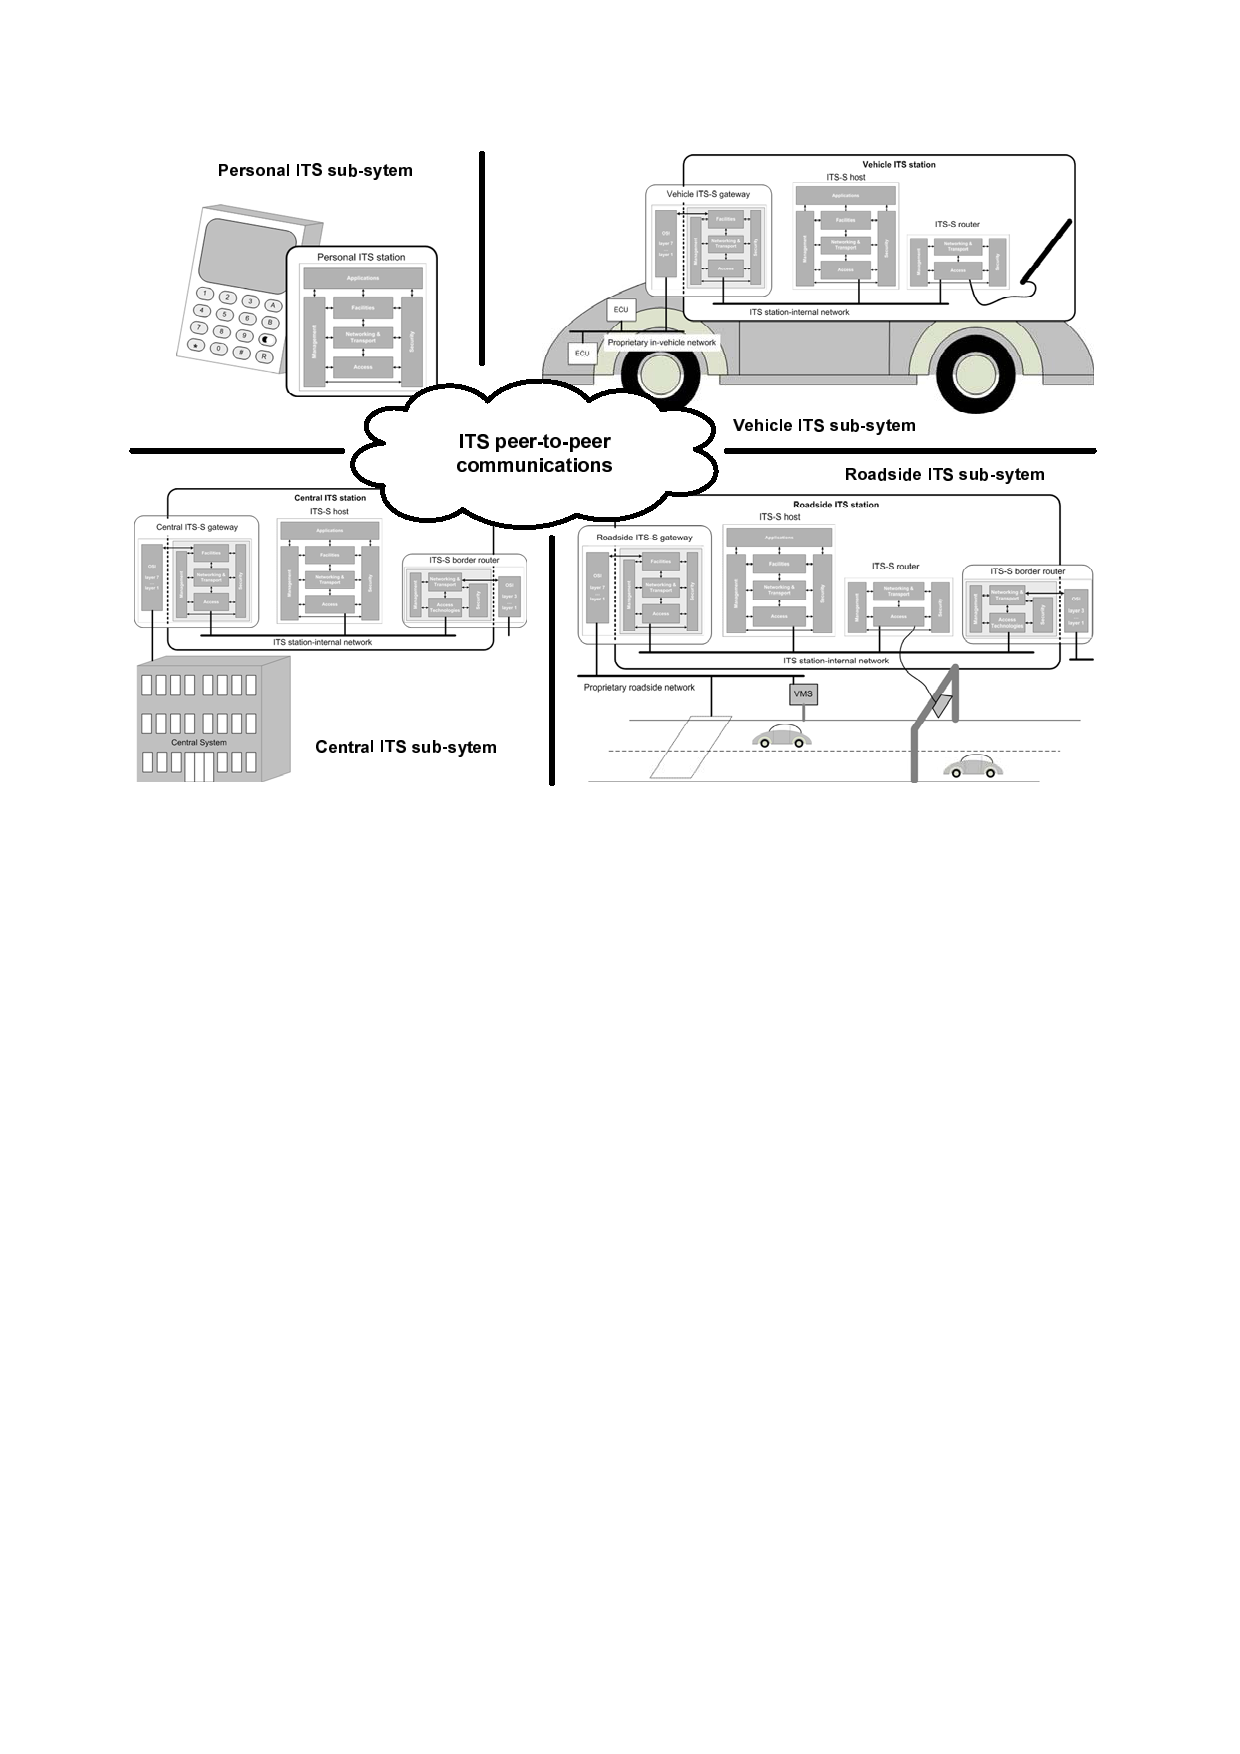
\includegraphics[width=0.99\textwidth]{content/images/01_funktionsweise/ueberblick-ITS-subsystems.pdf}
\caption{Überblick über die Komponenten \cite{etsi2010302}}
\label{fig:funktionsweise_komponentenueberblick}
\end{figure}

\section{Untereinheiten}
Die Untereinheiten sind sind in sich geschlossene Einheiten, die in den \ac{ITS} Komponenten vorhanden sind. Sie werden in diesem Abschnitt beschrieben. Zusätzlich werden die mindestens definierten Funktionalitäten genannt.
  
\subsection{Roadside ITS-S Gateway}
\subsection{ITS-S Host}
Der ITS-S Host beinhaltet mindestens die ITS-S Anwendungen und die Funktionalität der ITS  Station Reference Architektur, die für die  ITS-S Anwendungen gebraucht wird. 


\subsection{ITS-S Router}
\subsection{ITS-S Border Router}

\section{Personal subsystem and station}
\ac{PSS} stellen die Funktionalitäten von \ac{ITS} in Geräten zur Verfügung, die in der Hand gehalten werden können. Der Standard nennt hierzu \ac{PDA} oder Mobiltelefone als Beispiel. Sie können als eigenständige Komponente dienen, oder als Teil einer anderen Komponente arbeiten.

\section{ITS Central Station}
Die \ac{ICS}, oder Central \ac{ITS} subsystem and station ist eine zentrale Komponente im \ac{ITS} System. Sie bietet die Funktionalität an, um die Komponenten des zentralen Systems an das \ac{ITS} 

\section{ITS Roadside Station}
Die Kommunikation ist nicht auf die Kommunikation von Fahrzeugen untereinander beschränkt. Eine Kommunikation zwischen Fahrzeugen und Verkehrsinfrastruktur ist ebenfalls möglich. Diese Kommunikation wird über \ac{IRS} oder \ac{RSU} abgewickelt. Da sie den Informationsfluss zwischen \ac{IVS} und \ac{ICS} ermöglicht, hat sie einen hohen Stellenwert im System. \ac{IRS} werden im Normalfall in bereits vorhandene Infrastruktur integriert. Hierfür bieten sich beispielsweise Ampeln oder sonstige Verkehrsleitsysteme an. 

Die \ac{IRS} beherrscht zwei grundlegend unterschiedliche Verbindungsprotokolle. Über das verbindungslose ITS-G5 kann die \ac{IRS} Verbindungen zu den \ac{IVS} aufbauen. Die Verbindung zu den \ac{ICS} erfolgt über TCP/IP. 

Neben der Funktion als reine Schnittstelle zwischen \ac{IRS} und \ac{IVS} kann die \ac{IRS} die empfangenen Daten aufbereiten, bzw. ein FunctionFramework zur Verfügung stellen, auf dem Applikationen ausgeführt werden können.


Beispiele für Applikationen der \ac{IRS} sind:
\begin{itemize}
	\item Store and Forward von Ereignisinformationen \ac{DENM}.
	\item Weiterleitung von Ereignisinformationen an Versuchszentrale (Testzentrale)
	\item Aggregation von empfangenen Fahrzeugdaten zur Verbesserung der Wetter- und Verkehrslageerfassung. 
	\item Neue Anwendungen bzgl. der Interaktion zwischen Fahrzeug und LSA.
	\item  Kreuzungsassistenz sowie Assistenz im Baustellenbereich.
	\item Verteilung von Daten der ergänzenden Dienste aus der Versuchszentrale an die Fahrzeuge.
	\item Versendung von Daten zur Kreuzungstopologie.
\end{itemize}

Diese Beispiele sind aus einem Projektergebnis von \ac{SIMTD} entnommen (\cite{simtd-D12.1}). Im Standard sind die Funktionalitäten einer \ac{IRS} nicht genauer beschrieben. 




\section{IVS}


